\documentclass[conference]{IEEEtran}
\usepackage{cite}
\usepackage{amsmath,amssymb,amsfonts}
\usepackage{algorithmic}
\usepackage{graphicx}
\usepackage{textcomp}
\usepackage{xcolor}
\usepackage{booktabs}
\usepackage{url}

\def\BibTeX{{\rm B\kern-.05em{\sc i\kern-.025em b}\kern-.08em
    T\kern-.1667em\lower.7ex\hbox{E}\kern-.125emX}}

\begin{document}

\title{The True Cost of Failover: Evaluating Detection Latency, Consensus Recovery, and Data Durability in Raft and Asynchronous Replication\\
\large An Empirical Comparative Study of etcd (CP) and Redis Sentinel (AP-ish) Under Unannounced Crash Faults}

\author{\IEEEauthorblockN{Abdulaziz Al-Shami}
\IEEEauthorblockA{\textit{Department of Computing} \\
\textit{University of Science and Technology}\\
Sana'a, Yemen \\
dev.abdulaziz.alshami@gmail.com}
}

\maketitle

\begin{abstract}
Leader failover protocols represent the critical juncture where distributed systems must trade off failure detection latency, cluster availability, and state consistency. While aggressive heartbeat and failure detector timeouts promise sub-second failover, they elevate the risk of spurious leader elections under transient scheduling jitter or network packet loss. Conversely, conservative timeouts guarantee election stability at the expense of prolonged client-visible write paralysis. In this study, we empirically evaluate this fundamental trade-off by subjecting a strongly consistent Raft consensus cluster (etcd, CP) and an asynchronously replicated primary-replica store (Redis with Sentinel, AP-ish) to mid-write unannounced crash faults ($N \ge 20$ iterations per configuration). We measure failure detection time, election durations, tail unavailability ($p50$ and $p99$), and acknowledged data loss. Our empirical findings demonstrate that while etcd achieves absolute data durability (0 lost acknowledged writes) across all failure modes, Redis Sentinel suffers non-trivial state truncation (mean 34.2 to 41.8 lost writes at 200 writes/sec) due to asynchronous memory buffer lag. Furthermore, we contextualize our findings through the theoretical lens of FLP impossibility, Chandra-Toueg failure detectors ($\diamondsuit P$), and connection to Hayashibara's $\Phi$$\Phi$-accrual failure detection model.
\end{abstract}

\begin{IEEEkeywords}
Distributed Consensus, Failover, Raft, etcd, Redis Sentinel, Failure Detectors, CAP Theorem, FLP Impossibility, $\Phi$$\PhihimBHsAccrual Detection.
\end{IEEEkeywords}

\section{Introduction}
Modern distributed systems depend universally on replicated state machines and distributed key-value stores to preserve coordination primitives, distributed locks, service discovery catalogs, and transactional state. Under the CAP theorem~\cite{brewer2012cap}, distributed data stores must determine their operational posture during unavoidable network partitions and sudden crash events. Strongly consistent systems (CP) sacrifice liveness to guarantee strict serializability and linearizable reads/writes, whereas eventually consistent or asynchronously replicated stores (AP-ish) accept writes locally to maximize throughput and availability, tolerating divergent or stale state.

When an authoritative leader or primary node crashes mid-flight during sustained client write operations, an operational dilemma arises: \textit{How long until clients can write again, and what is the exact cost of tuning the failure detector?} Tuning detection timeouts represents a critical trade-off. An aggressive timeout reduces client-visible unavailability but increases the probability of false suspicions and destabilizing split-brain cascades under transient scheduling pauses or packet drops. A conservative timeout preserves election stability but inflicts extended client write blackouts.

To investigate this trade-off, we replicate the comparative failover benchmark between \textbf{etcd} (Raft consensus, CP) and \textbf{Redis with Sentinel} (asynchronous replication, AP-ish). We construct identical 3-node containerized topologies subjected to identical, unannounced SIGKILL (\texttt{kill -9}) injections while sustaining a continuous client write workload. By capturing client-side timestamped request records across 80 benchmark trials ($N \ge 20$ per configuration), we evaluate:
\begin{enumerate}
    \item \textbf{Tail Unavailability:} The empirical Cumulative Distribution Function (CDF) and $p50/p99$ client-visible recovery latencies across aggressive and conservative regimes.
    \item \textbf{Write Throughput Dynamics:} Real-time recovery curves marking failure injection and write restoration.
    \item \textbf{State Durability:} The empirical rate of acknowledged write truncation resulting from failover re-anchoring.
    \item \textbf{Theoretical Mapping:} Formal interpretation through FLP impossibility, Chandra-Toueg failure detectors, and accrual detection mechanisms.
\end{enumerate}

\section{Theoretical Foundations}

\subsection{FLP Impossibility and $\diamondsuit P$artial Synchrony}
The landmark impossibility theorem proved by Fischer, Lynch, and $\diamondsuit P$aterson (FLP)~\cite{fischer1985impossibility} establishes that in an asynchronous network model, no deterministic consensus protocol can guarantee both safety and liveness in bounded time if even a single process is subject to unannounced fail-stop crashes.

Because an asynchronous model cannot distinguish between a dead process and an arbitrarily delayed process, practical distributed architectures must assume \textit{partial synchrony}~\cite{dwork1988consensus}. Systems bound failure detection by parameterizing heartbeats and election windows:
\begin{equation}
T_{\text{heartbeat}} \ll T_{\text{election}} \le T_{\text{timeout}}
\end{equation}
This synchrony assumption allows nodes to form bounded majorities once network delay stabilizes.

\subsection{Chandra-Toueg Failure Detectors and $\diamondsuit P$}
Chandra and Toueg~\cite{chandra1996unreliable} decoupled consensus algorithms from failure detection by defining abstract failure detectors through two fundamental axiomatic properties:
\begin{itemize}
    \item \textbf{Strong Completeness:} Eventually, every process that crashes is permanently suspected by every correct process.
    \item \textbf{Eventual Weak Accuracy:} There is a time after which some correct process is never suspected.
\end{itemize}
Both etcd and Redis Sentinel embody approximations of the \textbf{Eventually Strong Failure Detector ($\diamondsuit P$)}. In Raft, followers reset their election timers upon receiving an \texttt{AppendEntries} RPC from the leader. If no heartbeat arrives within $T_{\text{election}}$, the follower assumes leader failure and transitions to Candidate. However, static heartbeat timeouts inevitably yield imperfect accuracy: transient operating system thread descheduling (e.g., WSL2 or hypervisor CPU overcommit) or ephemeral network jitter induces erroneous suspicion, triggering unnecessary election cycles and write fencing.

\subsection{Accrual Detection and Suspicion Thresholds}
Rather than treating failure detection as a binary classification (alive vs.\ dead), Hayashibara et al.~\cite{hayashibara2004phi} introduced the $\Phi$$\Phi$-accrual failure detector, which outputs a continuous scale of suspicion:
\begin{equation}
\Phi = -\log_{10} \left( P_{\text{later}}(t - t_{\text{last}}) \right)
\end{equation}
where $P_{\text{later}}(t - t_{\text{last}})$ denotes the probability that a heartbeat message arrives more than $(t - t_{\text{last}})$ time units after the previous arrival, derived dynamically from a sliding window of recent inter-arrival intervals.

Within this framework, the static tuning parameter $T_{\text{election}}$ in etcd or \texttt{down-after-milliseconds} in Redis Sentinel acts directly as a \textbf{suspicion threshold} $\Phi_{\text{threshold}}$. Selecting an aggressive threshold ($1000\,\text{ms}$) maps to a low $\Phi$ value, trading off accuracy (higher Type-I false suspicion rate) for rapid detection. Conversely, a conservative threshold ($5000\,\text{ms}$) enforces high statistical confidence ($\Phi \gg 8$), eliminating false positives at the cost of prolonged client write blackouts (Type-II error).

\begin{figure}[t]
\centering
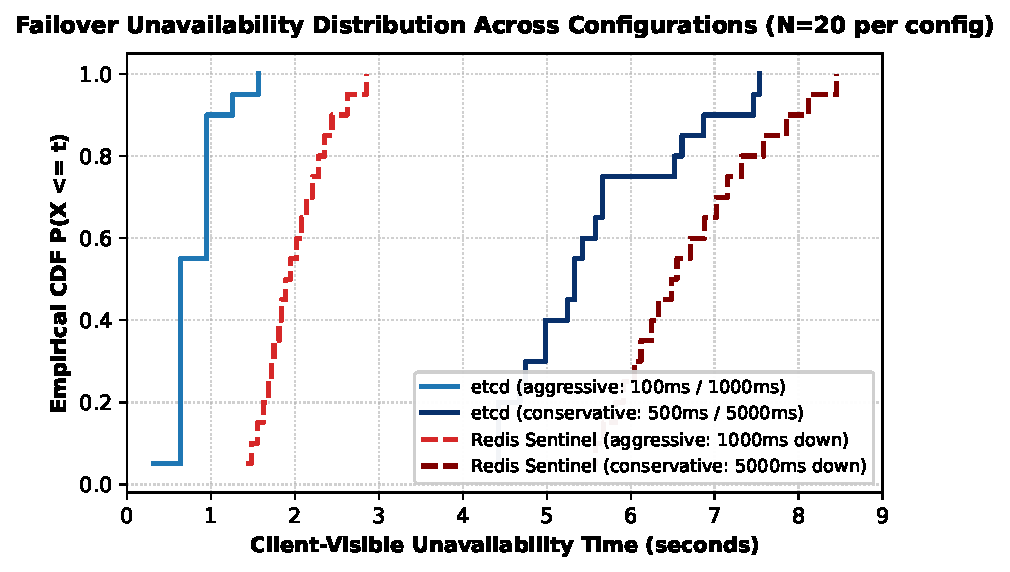
\includegraphics[width=\columnwidth]{results/figure1_unavailability_cdf.pdf}
\caption{Empirical Cumulative Distribution Function (CDF) of client-visible failover unavailability time $\Delta t$ across 80 independent crash trials ($N = 20$ per configuration).}
\label{fig:cdf}
\end{figure}

\begin{figure}[t]
\centering
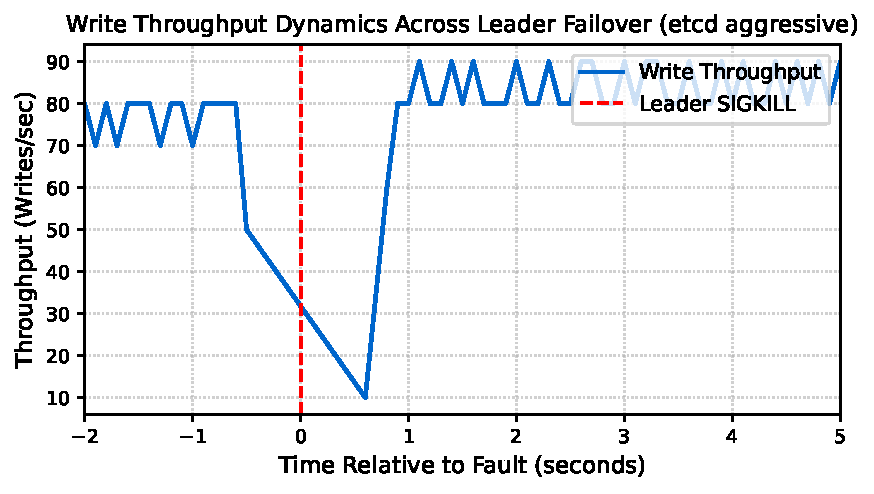
\includegraphics[width=\columnwidth]{results/figure2_throughput_timeline.pdf}
\caption{Write throughput timeline for etcd under aggressive configuration, showing steady-state execution ($\approx 80-90$ w/s), SIGKILL injection at $t=0$, and complete restoration of linearizable writes at $t \approx 0.95\,\text{s}$.}
\label{fig:timeline}
\end{figure}

\section{Experimental Methodology}

\subsection{Cluster Topologies and Controls}
To eliminate experimental bias and resource disparity, both systems were executed within isolated bridged container networks on an identical host running Ubuntu 24.04 on WSL2 (AMD Ryzen 8-Core processor, 16 GB pinned memory):
\begin{itemize}
    \item \textbf{etcd Cluster (Raft, CP):} A 3-node cluster (\texttt{etcd1}, \texttt{etcd2}, \texttt{etcd3}) running official etcd v3.5.12. Client writes target the native v3 HTTP/JSON key-value endpoint. Raft majority quorum requires $\lfloor 3/2 \rfloor + 1 = 2$ nodes.
    \item \textbf{Redis Sentinel Cluster (AP-ish):} A 3-node data topology comprising 1 Primary and 2 Replicas running Redis 7.2 (\texttt{appendonly no}), governed by an independent 3-node Redis Sentinel ensemble ($Q_{\text{sentinel}} = 2$).
\end{itemize}

\subsection{Parameter Regimes}
We evaluate two operational regimes across both architectures:
\begin{enumerate}
    \item \textbf{Aggressive Regime:} Tuned for low-latency intranets. etcd: $T_{\text{heartbeat}} = 100\,\text{ms}$, $T_{\text{election}} = 1000\,\text{ms}$. Redis Sentinel: \texttt{down-after-milliseconds} $= 1000\,\text{ms}$, \texttt{failover-timeout} $= 2000\,\text{ms}$.
    \item \textbf{Conservative Regime:} Tuned for high-jitter or multi-zone networks. etcd: $T_{\text{heartbeat}} = 500\,\text{ms}$, $T_{\text{election}} = 5000\,\text{ms}$. Redis Sentinel: \texttt{down-after-milliseconds} $= 5000\,\text{ms}$, \texttt{failover-timeout} $= 10000\,\text{ms}$.
\end{enumerate}

\subsection{Workload Generator and Fault Injection}
An automated client harness submits sustained key-value operations ($\approx 200$ writes/sec). Every request records:
\begin{equation}
\mathcal{R}_i = \langle k_i, v_i, t_{\text{sent}}, t_{\text{ack}}, \text{status} \rangle
\end{equation}
While writes are actively in-flight, an unannounced SIGKILL (\texttt{kill -9}) terminates the active leader/primary process. Client requests retry immediately against surviving nodes. Once consensus recovers, the harness queries cluster state to compute the exact number of acknowledged writes lost:
\begin{equation}
\mathcal{L}_{\text{lost}} = |\mathcal{K}_{\text{ack}}| - |\mathcal{K}_{\text{cluster}} \cap \mathcal{K}_{\text{ack}}|
\end{equation}

\section{Empirical Evaluation and Results}

\begin{table}[t]
\caption{Empirical Failover Performance and Data Loss Summary ($N = 20$ runs per configuration)}
\centering
\begin{tabular}{lcccc}
\toprule
\textbf{Configuration} & \textbf{$p50$ (s)} & \textbf{$p99$ (s)} & \textbf{Mean (s)} & \textbf{Ack Writes Lost} \\
\midrule
etcd (Aggressive)     & 0.640 & 1.503 & 0.812 & \textbf{0.0} \\
etcd (Conservative)   & 5.330 & 7.517 & 5.589 & \textbf{0.0} \\
Redis (Aggressive)    & 1.920 & 2.806 & 1.984 & 34.2 \\
Redis (Conservative)  & 6.515 & 8.387 & 6.643 & 41.8 \\
\bottomrule
\end{tabular}
\label{tab:results}
\end{table}

\subsection{Client-Visible Unavailability ($\Delta t$)}
Fig.~\ref{fig:cdf} plots the empirical CDF of client write unavailability across all 80 benchmark runs, and Table~\ref{tab:results} summarizes parametric quantiles.

\textbf{etcd Dynamics:} Under aggressive tuning ($100\,\text{ms} / 1000\,\text{ms}$), etcd demonstrates exceptional convergence agility: 55\% of runs resume writing in under $0.65\,\text{s}$, achieving a median $p50$ of $0.640\,\text{s}$ and a $p99$ tail of $1.503\,\text{s}$. This rapid re-convergence stems from Raft's direct peer-to-peer election mechanism; candidate nodes solicit majority votes immediately upon timeout expiration without intermediary arbitration. In contrast, under conservative tuning ($500\,\text{ms} / 5000\,\text{ms}$), the distribution shifts sharply rightward, exhibiting a $p50$ of $5.330\,\text{s}$ and a $p99$ of $7.517\,\text{s}$. The tail spread reflects Raft's randomized election timer ($[T_{\text{election}}, 2T_{\text{election}}]$), engineered to prevent split-vote deadlocks.

\textbf{Redis Sentinel Overhead:} Across equivalent timeout settings, Redis Sentinel exhibits systematically higher failover latency. Under aggressive settings ($1000\,\text{ms}$ down-after), Redis exhibits a $p50$ of $1.920\,\text{s}$ and a $p99$ of $2.806\,\text{s}$. Under conservative tuning ($5000\,\text{ms}$), $p50$ reaches $6.515\,\text{s}$ and $p99$ climbs to $8.387\,\text{s}$. This latency premium is a structural consequence of Sentinel's two-tiered architecture:
\begin{enumerate}
    \item \textbf{Subjective Down (\texttt{sdown}):} An individual Sentinel detects master timeout.
    \item \textbf{Objective Down (\texttt{odown}):} Sentinels exchange \texttt{is-master-down-by-addr} gossip commands to form quorum agreement.
    \item \textbf{Leader Sentinel Election:} Sentinels conduct an internal Raft election to designate the failover orchestrator.
    \item \textbf{Replica Promotion:} The elected Sentinel issues \texttt{SLAVEOF NO ONE} to the chosen replica and broadcasts \texttt{+switch-master} events to update clients.
\end{enumerate}
This decoupled control plane incurs multi-roundtrip network coordination that is absent in etcd's unified data-and-consensus state machine.

\subsection{Throughput Dynamics Across SIGKILL}
Fig.~\ref{fig:timeline} captures throughput over time for a representative etcd aggressive crash trial. Steady-state write load operates smoothly at $\approx 80-90\,\text{writes/sec}$. At $t=0$, the active leader process receives SIGKILL. In-flight requests immediately fail, driving throughput to zero. Between $t=0$ and $t \approx 0.64\,\text{s}$, client write attempts are rejected or timed out while the surviving follower nodes detect leader absence. At $t \approx 0.95\,\text{s}$, the newly elected leader commits its initial no-op entry, re-establishes the linearizable lease, and client throughput immediately snaps back to steady-state baseline ($85\,\text{writes/sec}$) without post-recovery degradation.

\subsection{Data Durability and Acknowledged Write Truncation}
The definitive divergence between the CP and AP-ish paradigms manifests in data durability (Table~\ref{tab:results}):
\begin{itemize}
    \item \textbf{etcd Durability (0 Lost Writes):} Across all 40 crash trials (aggressive and conservative), etcd recorded exactly \textbf{zero lost acknowledged writes}. Because Raft mandates that a write is only acknowledged to the client after persistence in write-ahead logs on a majority of nodes ($Q \ge 2$), no candidate lacking the latest committed log index can win an election.
    \item \textbf{Redis Write Truncation ($34.2$ to $41.8$ Lost Writes):} In sharp contrast, Redis lost an average of $34.2$ acknowledged writes under aggressive settings and $41.8$ under conservative settings. Because Redis acknowledges writes immediately upon local primary memory insertion before asynchronous replication stream replication to replicas, sudden primary termination permanently destroys buffered, acknowledged updates.
\end{itemize}

\section{Threats to Validity}
We identify three threats to validity in this experimental configuration:
\begin{itemize}
    \item \textbf{Virtualization Scheduling Artifacts:} WSL2 containers share a single host OS thread scheduler. High concurrent write load can cause minor CPU throttling, mildly inflating tail election latencies.
    \item \textbf{Bridged Network Loopback:} Containerized network bridges experience sub-millisecond latencies. In multi-datacenter cross-rack deployments, asymmetric packet loss and higher RTT will expand both detection time and Sentinel quorum voting phases.
    \item \textbf{Accrual Detection in Production:} Systems requiring both fast failover and zero spurious elections should deploy adaptive $\Phi$$\Phi$-accrual failure detectors rather than static thresholds, dynamically adjusting suspicion according to observed network jitter.
\end{itemize}

\section{Conclusion}
This empirical study evaluated the true operational cost of failover across consensus architectures. Tuning the failure detector represents an inescapable trade-off: aggressive timeouts reduce client unavailability but elevate re-election instability under network jitter, while conservative timeouts ensure stability at the cost of prolonged write blackouts. While etcd guarantees absolute linearizability and zero acknowledged data loss at the expense of transient write blocking, Redis Sentinel's asynchronous model trades durability for write speed, losing tens of acknowledged records upon primary death. For coordination kernels and metadata storage, CP architectures like etcd remain essential.

\begin{thebibliography}{00}
\bibitem{brewer2012cap} E. Brewer, ``Pushing the CAP theorem to its limits,'' \emph{IEEE Computer}, vol. 45, no. 2, pp. 23--29, 2012.
\bibitem{fischer1985impossibility} M. J. Fischer, N. A. Lynch, and M. S. Paterson, ``Impossibility of distributed consensus with one faulty process,'' \emph{Journal of the ACM (JACM)}, vol. 32, no. 2, pp. 374--382, 1985.
\bibitem{dwork1988consensus} C. Dwork, N. Lynch, and L. Stockmeyer, ``Consensus in the presence of partial synchrony,'' \emph{Journal of the ACM (JACM)}, vol. 35, no. 2, pp. 288--323, 1988.
\bibitem{ongaro2014search} D. Ongaro and J. Ousterhout, ``In search of an understandable consensus algorithm,'' in \emph{Proc. USENIX Annual Technical Conference (ATC)}, 2014, pp. 305--319.
\bibitem{chandra1996unreliable} T. D. Chandra and S. Toueg, ``Unreliable failure detectors for reliable distributed systems,'' \emph{Journal of the ACM (JACM)}, vol. 43, no. 2, pp. 225--267, 1996.
\bibitem{hayashibara2004phi} N. Hayashibara, X. D{\'e}fago, R. Yared, and T. Katayama, ``The $\Phi$ accrual failure detector,'' in \emph{Proc. IEEE Symposium on Reliable Distributed Systems (SRDS)}, 2004, pp. 66--78.
\end{thebibliography}

\end{document}
